\section{In-situ thermal management, monitoring and annealing}
\label{sec:monitoring}

\subsection{Thermal architectures: chamber, plate and local heating}
Three architectures for managing the thermal history of the deposited glass are found in the corpus, and they map onto the three direct sub-families.

\emph{Whole-part chamber heating} (crucible-fed). The build chamber is held \SIrange{20}{40}{\celsius} below the annealing point so that every layer, once deposited, relaxes toward a state of near-zero stress while remaining rigid. Klein et al.\ documented the evolution: parts printed at room temperature and kept above \(\Tg\) with hand-held propane torches cracked frequently; the heated chamber eliminated cracking and the polariscope showed a homogeneous stress state without the radial intralayer stresses of cold-printed samples \citep{klein2015}. The chamber also removes the thermal shock at the build plate: a ceramic kiln-shelf plate bonds to the first layer at high temperature and releases it at the annealing temperature \citep{klein2015}, and preheated float-glass sheets can be used as the plate to produce rib-on-plate hybrids, provided the sheet is brought to just above its annealing point before printing \citep{stern2024cgc}. The cost is energy: \SI{12}{kW} for the G3DP2 chamber alone \citep{inamura2018}.

\emph{Heated build plate plus post-anneal} (laser filament, powder bed). The workpiece rests on a plate at \SIrange{250}{600}{\celsius}; the small melt zone cools within milliseconds to seconds, so the part accumulates residual stress in each layer and is annealed afterwards. This is tolerable for fused silica (\(\alpha = \SI{0.5e-6}{\per\kelvin}\)) and marginal for soda-lime; Datsiou et al.\ held the L-PBF substrate at \SI{250}{\celsius} explicitly to reduce thermal cracking \citep{datsiou2019}, and Spirrett et al.\ found substrate cracking unavoidable above \SI{115}{W} on \SI{1}{mm} float substrates in DED \citep{spirrett2023}. For fused silica the coaxial-beam LGD head was introduced precisely to lower residual stress by symmetric heating of the fibre \citep{lgd2021coaxial}.

\emph{Localised auxiliary heating} (all families). Torches and lasers are used as auxiliaries: G3DP2's concentric propane burner at the nozzle tip starts flow and the compressed-air ring stops it \citep{inamura2018}; Rammig's early all-glass connections were torch-melted soda-lime rod on plate \citep{rammig2012,seel2018}; and Notre Dame combines CO or CO$_2$ heating with ultrafast-laser machining in a hybrid station \citep{notredame_dgf}. No published molten-glass printer yet uses a secondary laser to preheat the previous layer immediately ahead of the nozzle, although this is standard in large-format polymer and metal DED and is an obvious transfer (\cref{sec:outlook}).

\subsection{Temperature sensing}
\paragraph{Thermocouples.} All kiln zones are controlled by type-K or type-S thermocouples with PID controllers; G3DP2 used a Watlow EZ-Zone with redundant sensors per zone and network connectivity \citep{inamura2018}; the patent specifies type-S at the nozzle for response speed \citep{patent_us9919510,klein2015}. Thermocouples measure the refractory, not the glass; the offset between nozzle-kiln set point (\SI{1010}{\celsius}) and glass exit temperature (\SI{920}{\celsius} measured, \SI{990}{\celsius} simulated) in G3DP illustrates the gap \citep{klein2015}.

\paragraph{Infrared thermography.} Glass has an emissivity close to unity in the long-wave infrared, so a thermal camera views the cord almost as a black body and is insensitive to reflections of the hot kiln. G3DP used a FLIR T335 with a high-temperature option through the Neoceram window to map a \SI{350}{\celsius} gradient across five layers \citep{klein2015}; G3DP3 uses an Optris PI 640i G7 at \SI{7.9}{\micro\metre} with an assumed emissivity of 0.98 to record the maximum cord temperature during printing (\SI{969}{\celsius} for Spruce Pine 87, \SI{1023}{\celsius} for Spruce Pine PWV, \SI{1045}{\celsius} for recycled container glass, \SI{1059}{\celsius} for Optifloat float glass) and to calibrate set points by comparing printed mass with predicted mass \citep{stern2024cgc}. The \SI{7.9}{\micro\metre} band is chosen because glass is opaque there, so the reading is a surface temperature; shorter-wave pyrometers see partly into the volume of a transparent melt.

\paragraph{Pyrometry and spectroscopy of laser melt pools.} Luo et al.\ monitored the incandescence of the filament melt pool with a spectrometer and a pyrometer; the spectrum revealed the onset of material breakdown and reboil bubbles at excessive temperature, and a low-order energy-balance model converted the signal into an estimated melt temperature suitable for feedback \citep{luo2017heat,luo2018quartz}. The IOE-CAS group closed the loop with a pyrometer and PID adjustment of laser power \citep{lgd2025tempctrl}.

\paragraph{Thermal imaging in the loop.} The 2026 digital-glass-forming controller integrates a thermal camera with deterministic real-time control on RT-Linux; the work-zone temperature must stay within the working range because too cool a zone does not bond and too hot a zone vaporises or detaches the filament, and the closed loop prevented both failure modes in multilayer walls that fail under constant power \citep{dgf2026control}. The transition from single-point pyrometry to spatial imaging is the most significant control advance of the period, because it allows the controller to see the temperature of the previous layer, not only of the melt.

\paragraph{Vision.} Cameras are used for process observation rather than control: the LGD platform has an on-axis process camera and a separate beam camera that images the wavefront transmitted through the finished specimen to detect bubbles and striae \citep{lgd2024homog}; G3DP2 relies on servo encoders for closed-loop position and reports axis faults to the interface so that the Z-axis can retract to protect the nozzle \citep{inamura2018}. Nobula advertises computer vision as part of its platform \citep{nobula_web}, but no peer-reviewed description of vision-based bead-width or slump control in molten glass exists in the corpus.

\subsection{Feed-rate and flow control}
In gravity-fed extrusion the flow rate is a slow function of head and nozzle temperature and cannot be modulated within a layer; the machine controls geometry instead through the travel speed. G3DP found that driving the bed \SI{7}{\percent} faster than the natural exit velocity produced the most uniform cord (the slight tension prevents glass accumulating at the nozzle), while the first layer was slowed by \SI{25}{\percent} to let the glass settle on the plate \citep{klein2015}. Bead width is then \(w = Q/(v_{\mathrm{travel}} h_{\mathrm{layer}})\), and any flow drift appears as a width change rather than a height change because the nozzle sets the layer height by direct contact \citep{klein2015}. G3DP3 encodes feed rate, bead height and bead width limits (\cref{sec:hardware}) in the toolpath generator, and the mass-prediction check after each print feeds back into set-point corrections of \SIrange{-10}{0}{\celsius} \citep{stern2024cgc}. Start and stop of flow remain the weakest link: neither G3DP2 nor G3DP3 can interrupt flow mid-object, so every part must be a single continuous path---a constraint that shaped the figure-eight masonry design \citep{mit2024masonry}---and the MIT patent's automated shears are the proposed remedy \citep{patent_us9919510}.

In filament and cane processes the feed motor sets the volumetric rate directly, and the controllable variables are feed rate, travel speed and laser power (or nozzle temperature). The KTH study maps bonding width against all three and shows a plateau in bonding width with power, which defines the robust operating point \citep{kth2022bonding}; the LGD study maps surface roughness and contour angle against feed rate and shows the trade-off between smoothness and geometric fidelity \citep{lgd2024homog}.

\subsection{Annealing schedules and stress verification}
\paragraph{Schedules.} G3DP annealed in the chamber after each print; G3DP2 soaked at \SI{525}{\celsius} and transferred to an external lehr; G3DP3 uses multi-hour programmed cycles, with the fully printed masonry units (thick printed bases) given longer cycles than hollow units, and print-cast units reheated to the annealing point (\SI{500}{\celsius}) before ladling molten glass into them to avoid thermal shock \citep{klein2015,inamura2018,mit2024masonry}. L-PBF parts were post-treated at \SI{650}{\celsius} for five hours to improve translucency \citep{datsiou2019}. The physics is that of \cref{eq:stress}: hold at the annealing point until the through-thickness gradient has relaxed, then cool at a rate \(\dot{T} \lesssim 2k\,\Delta T_{\mathrm{allow}}/(\rho c_p \delta^{2})\) through the strain point, which for a \SI{13}{mm} wall and an allowable \(\Delta T\) of \SI{10}{\celsius} is a few \si{\celsius}/min.

\paragraph{Photoelastic verification.} Because glass is birefringent under stress, residual stress is inspected by polariscopy. Klein et al.\ used a 6-inch polariscope with a tint plate for a qualitative fringe reading and found negligible stress along the layers in both cold- and hot-printed samples after annealing, but unrelieved radial stress within the layers of cold-printed samples \citep{klein2015}. The KTH group reported no stress-induced birefringence in 105-layer fused-silica walls \citep{kth2022bonding}. Quantitative techniques---integrated photoelasticity for axisymmetric parts, photoelastic tomography for arbitrary shapes, scattered-light polariscopy for surface stress---are mature in the glass industry \citep{aben2008} but have not yet been applied systematically to printed glass; this is one of the open problems listed in \cref{sec:open}. Chemical tempering of G3DP2 cylinders produced strengths at both extremes of the range (\SIrange{39}{100}{MPa}) and was set aside in favour of annealed glass with a safety factor of ten, giving a design strength of \SI{4.1}{MPa} for the Milan columns \citep{inamura2018}.

\subsection{Reference: the KTH process map as an example of systematic characterisation}
\Cref{fig:kth} reproduces the experimental setup diagram of the KTH filament study under its CC-BY licence; it is included because it is the clearest published depiction of a laser-filament head with coaxial multi-beam heating and because the paper is the most complete process-window map in the direct-laser sub-family.

\begin{figure}[htbp]
  \centering
  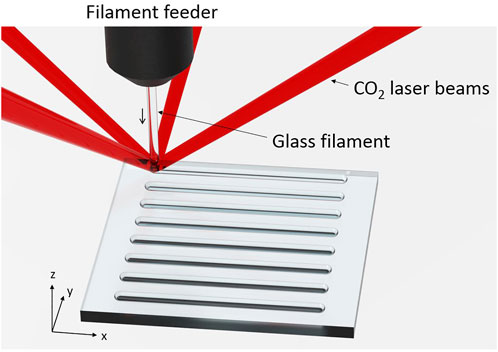
\includegraphics[width=0.8\linewidth]{kth2022_fig1.jpg}
  \caption{Filament-based glass 3D printing setup of Liu, Oriekhov and Fokine (KTH Royal Institute of Technology): a \SI{196}{\micro\metre} fused-silica filament is fed into a hot zone formed by four focused CO$_2$-laser beams above a fused-quartz build plate on a motion stage. Reproduced from \citet{kth2022bonding} (Frontiers in Materials, CC BY 4.0).}
  \label{fig:kth}
\end{figure}
